\documentclass[11pt]{article}
\usepackage[toc,page]{appendix}
\usepackage{amsmath, amssymb}
\usepackage[utf8]{inputenc}
\usepackage[T1]{fontenc}
\usepackage[style=apa,backend=biber]{biblatex}
%\usepackage{biblatex}
\addbibresource{references.bib}
\usepackage{graphicx}
\usepackage{tikz}
\usetikzlibrary{automata,positioning,shapes.geometric, arrows.meta, fit, backgrounds, calc, chains}
\graphicspath{./images/Easy_Pictures/SMR_MULT_Repackaging}%\usepackage{kpfonts}
\usepackage{float}
\usepackage[margin=1in]{geometry}
\usepackage{cancel}
\usepackage{epsfig}
\usepackage{tikz-3dplot}
\usepackage{darkmode}
\usepackage{dirtytalk}
\usepackage{longtable,booktabs,array}
\usepackage{calc} % for calculating minipage widths
\usepackage[utf8]{inputenc}
\usepackage[T1]{fontenc}
\usepackage{xcolor}
\usepackage{listings}


\usepackage{etoolbox}
\usepackage{hyperref}
\hypersetup{
 colorlinks=true,
 linkcolor=blue,
 filecolor=magenta, 
 urlcolor=cyan,
 pdftitle={Hermeneutic Calculator},
 citecolor=blue,
 }


\urlstyle{same}

\lstdefinestyle{htmlStyle}{
 language=HTML,
 basicstyle=\ttfamily\small,
 keywordstyle=\color{blue}\bfseries,
 commentstyle=\color{gray}\itshape,
 stringstyle=\color{red},
 breaklines=true,
 frame=single,
 numbers=left,
 numberstyle=\tiny\color{gray},
 columns=fullflexible,
}
\lstdefinelanguage{HTML}{
 keywords={<!DOCTYPE, html, head, title, body, h1, h2, h3, p, div, span, a, img, ul, li, table, tr, td, th, style, link, script},
 sensitive=true,
 comment=[l]{//},
 morecomment=[s]{/*}{*/},
 morestring=[b]',
 morestring=[b]"
}
\lstset{style=htmlstyle, language=html}
% Updated to explicitly pass the language option
%\lstinputlisting[style=htmlstyle, language=html]{./html/example.html}
%\usepackage{tocloft}

% Optional: define some custom colors
\definecolor{sliceRed}{RGB}{225,224,91} % matching "varyellow" from your code
\definecolor{linkYellow}{RGB}{255,215,0} % a golden yellow
\tdplotsetmaincoords{70}{110}

\title{Subtraction Strategies: Decomposition}
\author{Compiled by: Theodore M. Savich}

\begin{document}
\maketitle
\subsection*{Transcript}
Video from \textcite{Carpenter1999}. Strategy descriptions and examples adapted from \textcite{HackenbergCourseNotes}
\begin{itemize}
      \item \textbf{Teacher:} Lucy ordered 45 cupcakes for her birthday. At the party, her guests ate 27 cupcakes, how many cupcakes did she have left? [BACKGROUND] 
      \item \textbf{Joel:} This is 10, this is 10, this is 10, this is 10 and this is five.18. 
      \item \textbf{Teacher:} Explain to us what you did there. 
      \item \textbf{Joel:} I have, this is 10, this is 10, this is 10, and this is five. So I take away 20 and I take away five. I take away two more. So they enter and then I counted these and those, and so the answer was 18. 
      \item \textbf{Teacher:} Nice work
\end{itemize}
 
\noindent \textbf{Notation Representing Joel's Solution:}
\begin{align*}
      47-27 & \\
      45 - 20 &=25 \\
      25 - 7 &= ?\\
      &2 \text{ tens } + 5 \text{ ones } - 7 \text{ ones } \\
      1 \text{ ten } + &1 \text{ ten } + 5 \text{ ones } - 7 \text{ ones } \\
                             &\downarrow \text{DECOMPOSE}\\
      1 \text{ ten } + &10 \text{ ones }+5 \text{ ones } - 7 \text{ ones } \\ 
      &1 \text{ ten } + 8 \text{ ones }+\underbrace{7 \text{ ones }- 7 \text{ ones }}_{=0}\\ 
      %									&=0 \\
      &1 \text{ ten } + 8 \text{ ones } 
      \end{align*}
      

      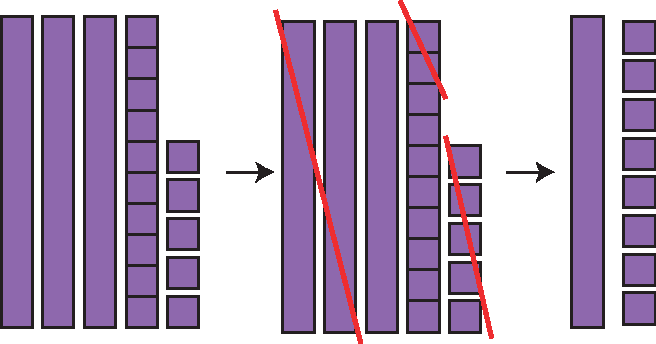
\includegraphics[width=.8\textwidth]{images/Easy_Pictures/SAR_SUB_Decomposition/PDF/SAR_SUB_Decomposition.pdf}

      \noindent \textbf{Notation Representing Joel's Solution:}
      \noindent Imagine representing both numbers by their base units and ones. Begin by subtracting the base components, then subtract the ones. If there aren't enough ones available in the larger number to subtract the ones from the smaller number (while keeping the result positive), break one base unit into its individual ones. Finally, remove only the exact number of ones required to complete the subtraction.


\subsection*{Decomposition}

\subsubsection*{Description of Strategy}
\begin{itemize}
    \item \textbf{Objective:} Decompose a base unit from the minuend into ones to have enough ones to subtract the ones in the subtrahend.
\end{itemize}

\subsubsection*{Corrected Automaton (Register Machine Model)}

We define a Register Machine that accurately models Joel's Left-to-Right cognitive sequence. This model is simplified for two digits (Tens and Ones) to match the example, assuming M >= S.

**M = (Q, V, \delta, q_0, F)**

\begin{itemize}
    \item \textbf{States (Q):} {$q_{init}, q_{sub\_bases}, q_{check\_ones}, q_{decompose}, q_{sub\_ones}, q_{accept}$}
    \item \textbf{Registers (V):} S\_T/S\_O (Subtrahend Tens/Ones), R\_T/R\_O (Result/Working Memory Tens/Ones).
\end{itemize}

**Transition Function (\delta):**

\begin{longtable}{|l|l|l|l|l|}
\hline
\textbf{Current State} & \textbf{Condition} & \textbf{Next State} & \textbf{Action} & \textbf{Interpretation} \\
\hline
\endhead
$q_{init}$ & - & $q_{sub\_bases}$ & Decompose S (S\_T/O). Init R=M (R\_T/O). & Initialize place values. \\
\hline
$q_{sub\_bases}$ & - & $q_{check\_ones}$ & R\_T -= S\_T & Subtract the bases (Tens). \\
\hline
$q_{check\_ones}$ & **R\_O >= S\_O** & $q_{sub\_ones}$ & - & Sufficient ones. \\
\hline
$q_{check\_ones}$ & **R\_O < S\_O** & $q_{decompose}$ & - & Insufficient ones. \\
\hline
$q_{decompose}$ & R\_T > 0 & $q_{sub\_ones}$ & R\_T -= 1; R\_O += Base & Decompose (borrow) one ten. \\
\hline
$q_{sub\_ones}$ & - & $q_{accept}$ & R\_O -= S\_O & Subtract the ones. \\
\hline
\end{longtable}

\subsubsection*{Automaton Diagram for Decomposition}

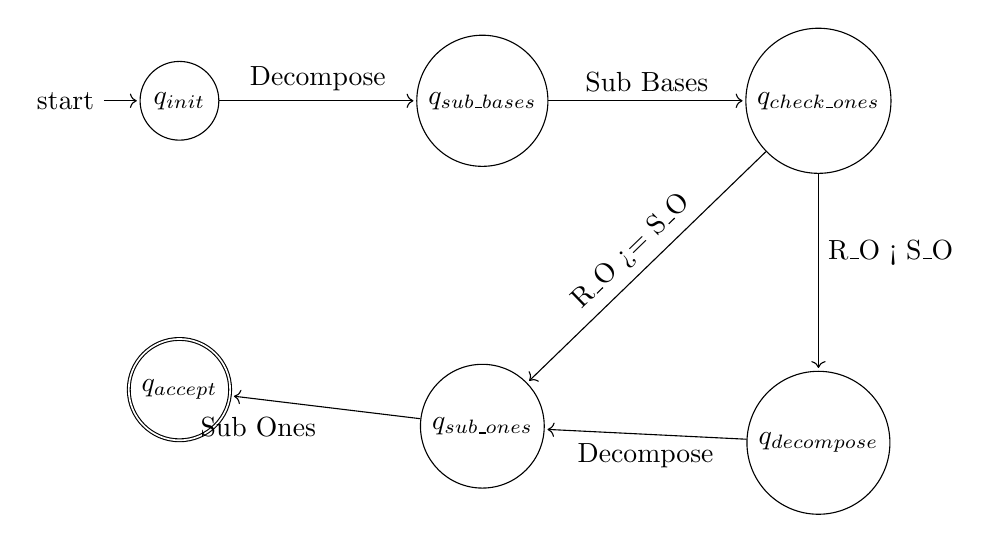
\begin{tikzpicture}[
    shorten >=1pt,
    auto,
    node distance=2.5cm,
    every state/.style={minimum size=1cm, align=center}
]
    % States
    \node[state, initial] (init) {$q_{init}$};
    \node[state, right=of init] (sub_bases) {$q_{sub\_bases}$};
    \node[state, right=of sub_bases] (check_ones) {$q_{check\_ones}$};
    \node[state, below=of check_ones] (decompose) {$q_{decompose}$};
    \node[state, below=of sub_bases] (sub_ones) {$q_{sub\_ones}$};
    \node[state, accepting, below=of init] (accept) {$q_{accept}$};

    % Transitions
    \path[->]
        (init) edge node {Decompose} (sub_bases)
        (sub_bases) edge node {Sub Bases} (check_ones)
        (check_ones) edge node[pos=0.4] {R\_O < S\_O} (decompose)
        (check_ones) edge node[sloped, above] {R\_O >= S\_O} (sub_ones)
        (decompose) edge node {Decompose} (sub_ones)
        (sub_ones) edge node {Sub Ones} (accept);
\end{tikzpicture}

\subsubsection*{Python Implementation and Test}

\begin{lstlisting}[language=Python]
import pandas as pd

class DecompositionAutomaton:
    """
    A Register Machine model simulating the 'Decomposition' (Borrowing) strategy for subtraction.
    Models the Left-to-Right approach: Subtract bases first, then ones, decomposing if necessary.
    """
    def __init__(self, M, S, Base=10):
        self.M = M
        self.S = S
        self.Base = Base
        self.state = 'q_start'
        self.history = []
        self.Result = 0

        # Registers for place values (Simplified for 2 digits based on the example)
        # S=Subtrahend (Reference), R=Result (Working Memory); T=Tens, O=Ones
        self.S_T = 0; self.S_O = 0
        self.R_T = 0; self.R_O = 0

        if S > M:
            self.state = 'q_error'
            self._record_history(f"Error: Subtrahend ({S}) > Minuend ({M}).")

    def _record_history(self, interpretation, highlight=False):
        self.history.append({
            'State': self.state, 'Interpretation': interpretation,
            'R_Tens': self.R_T, 'R_Ones': self.R_O,
            'Highlight': highlight
        })

    def transition(self, next_state):
        self.state = next_state

    def run(self):
        while self.state not in ['q_accept', 'q_error']:
            executor = getattr(self, f"execute_{self.state}", self.execute_error)
            executor()
        return self.Result

    def execute_error(self):
        if self.state != 'q_error':
            self._record_history(f"Error: Entered unknown state {self.state}")
            self.transition('q_error')

    # --- State Execution Methods ---

    def execute_q_start(self):
        self._record_history(f"Inputs: M={self.M}, S={self.S}", highlight=True)
        self.transition('q_init')

    def execute_q_init(self):
        """Decompose M and S into Tens and Ones."""
        # Decompose S for reference
        self.S_T = self.S // self.Base; self.S_O = self.S % self.Base
        # Initialize Result registers to M components
        self.R_T = self.M // self.Base; self.R_O = self.M % self.Base

        self._record_history(f"Decompose M ({self.R_T}T+{self.R_O}O) and S ({self.S_T}T+{self.S_O}O).")
        self.transition('q_sub_bases')

    def execute_q_sub_bases(self):
        """Subtract the bases (Tens)."""
        Initial_R_T = self.R_T
        # In this L-to-R approach, we subtract the tens first.
        self.R_T -= self.S_T
        self._record_history(f"Subtract Bases: {Initial_R_T}T - {self.S_T}T = {self.R_T}T.", highlight=True)
        self.transition('q_check_ones')

    def execute_q_check_ones(self):
        """Check if there are enough ones to subtract."""
        if self.R_O >= self.S_O:
            self._record_history(f"Sufficient Ones ({self.R_O} >= {self.S_O}). Proceed.")
            self.transition('q_sub_ones')
        else:
            self._record_history(f"Insufficient Ones ({self.R_O} < {self.S_O}). Need decomposition.", highlight=True)
            self.transition('q_decompose')

    def execute_q_decompose(self):
        """Decompose (borrow) one ten into ones."""
        if self.R_T > 0:
            self.R_T -= 1
            self.R_O += self.Base
            self._record_history(f"Decomposed 1 Ten. New state: {self.R_T}T, {self.R_O}O.", highlight=True)
            self.transition('q_sub_ones')
        else:
            # Should be unreachable if M>=S
            self.transition('q_error')

    def execute_q_sub_ones(self):
        """Subtract the ones."""
        prev_O = self.R_O
        self.R_O -= self.S_O
        self._record_history(f"Subtract Ones: {prev_O}O - {self.S_O}O = {self.R_O}O.", highlight=True)
        self.transition('q_accept')

    def execute_q_accept(self):
        """Combine results."""
        self.Result = self.R_T * self.Base + self.R_O
        self._record_history(f"Accept. Final Result: {self.Result}.", highlight=True)

    def display_history(self, summarized=True):
        print(f"\n--- Decomposition (L-to-R) Execution History ({self.M} - {self.S}) ---")
        df = pd.DataFrame(self.history)
        display_cols = ['State', 'Interpretation', 'R_Tens', 'R_Ones']

        if summarized:
             print("Summary Trace:")
             summary_df = df[df['Highlight'] == True]
             if not summary_df.empty:
                print(summary_df[display_cols].to_markdown(index=False))
        else:
            print("Full Trace:")
            print(df[display_cols].to_markdown(index=False))

# Test Case 1: Joel's example (45 - 27) - Requires Decomposition
print("=== Test Case 1: 45 - 27 (Requires Decomposition) ===")
decomp_45_27 = DecompositionAutomaton(M=45, S=27)
decomp_45_27.run()
decomp_45_27.display_history(summarized=False)

# Test Case 2: No decomposition needed (48 - 23)
print("\n=== Test Case 2: 48 - 23 (No Decomposition Needed) ===")
decomp_48_23 = DecompositionAutomaton(M=48, S=23)
decomp_48_23.run()
decomp_48_23.display_history(summarized=True)
\end{lstlisting}

\subsubsection*{Execution Trace (45 - 27):}
\begin{verbatim}
--- Decomposition (L-to-R) Execution History (45 - 27) ---
Full Trace:
| State         | Interpretation                                          |   R_Tens |   R_Ones |
|:--------------|:--------------------------------------------------------|---------:|---------:|
| q_start       | Inputs: M=45, S=27                                      |        0 |        0 |
| q_init        | Decompose M (4T+5O) and S (2T+7O).                      |        4 |        5 |
| q_sub_bases   | Subtract Bases: 4T - 2T = 2T.                           |        2 |        5 |
| q_check_ones  | Insufficient Ones (5 < 7). Need decomposition.          |        2 |        5 |
| q_decompose   | Decomposed 1 Ten. New state: 1T, 15O.                   |        1 |       15 |
| q_sub_ones    | Subtract Ones: 15O - 7O = 8O.                           |        1 |        8 |
| q_accept      | Accept. Final Result: 18.                               |        1 |        8 |
\end{verbatim}

\printbibliography

\end{document}